


\tikzset{every picture/.style={line width=0.75pt}} %set default line width to 0.75pt        

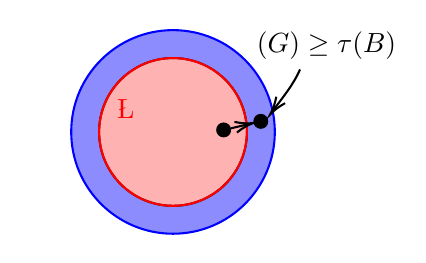
\begin{tikzpicture}[x=0.75pt,y=0.75pt,yscale=-1,xscale=1,scale=0.8]
%uncomment if require: \path (0,1301); %set diagram left start at 0, and has height of 1301

%Shape: Circle [id:dp47986660056185837] 
\draw  [color={rgb, 255:red, 0; green, 0; blue, 255 }  ,draw opacity=1 ][fill={rgb, 255:red, 0; green, 0; blue, 255 }  ,fill opacity=0.45 ] (223.39,1067.1) .. controls (223.39,1033.24) and (250.84,1005.79) .. (284.7,1005.79) .. controls (318.56,1005.79) and (346.01,1033.24) .. (346.01,1067.1) .. controls (346.01,1100.96) and (318.56,1128.41) .. (284.7,1128.41) .. controls (250.84,1128.41) and (223.39,1100.96) .. (223.39,1067.1) -- cycle ;
%Shape: Circle [id:dp35612564405295855] 
\draw  [fill={rgb, 255:red, 255; green, 255; blue, 255 }  ,fill opacity=1 ] (240.2,1067.1) .. controls (240.2,1042.52) and (260.12,1022.6) .. (284.7,1022.6) .. controls (309.28,1022.6) and (329.2,1042.52) .. (329.2,1067.1) .. controls (329.2,1091.68) and (309.28,1111.6) .. (284.7,1111.6) .. controls (260.12,1111.6) and (240.2,1091.68) .. (240.2,1067.1) -- cycle ;
%Shape: Circle [id:dp14338934667239034] 
\draw  [color={rgb, 255:red, 255; green, 0; blue, 0 }  ,draw opacity=1 ][fill={rgb, 255:red, 255; green, 0; blue, 0 }  ,fill opacity=0.3 ] (240.2,1067.1) .. controls (240.2,1042.52) and (260.12,1022.6) .. (284.7,1022.6) .. controls (309.28,1022.6) and (329.2,1042.52) .. (329.2,1067.1) .. controls (329.2,1091.68) and (309.28,1111.6) .. (284.7,1111.6) .. controls (260.12,1111.6) and (240.2,1091.68) .. (240.2,1067.1) -- cycle ;
%Shape: Circle [id:dp1521758257493362] 
\draw  [draw opacity=0][fill={rgb, 255:red, 0; green, 0; blue, 0 }  ,fill opacity=1 ][line width=0.75]  (310.7,1065.9) .. controls (310.7,1063.41) and (312.71,1061.4) .. (315.2,1061.4) .. controls (317.69,1061.4) and (319.7,1063.41) .. (319.7,1065.9) .. controls (319.7,1068.39) and (317.69,1070.4) .. (315.2,1070.4) .. controls (312.71,1070.4) and (310.7,1068.39) .. (310.7,1065.9) -- cycle ;
%Shape: Circle [id:dp00031221021643235147] 
\draw  [draw opacity=0][fill={rgb, 255:red, 0; green, 0; blue, 0 }  ,fill opacity=1 ][line width=0.75]  (333.07,1060.73) .. controls (333.07,1058.25) and (335.08,1056.23) .. (337.57,1056.23) .. controls (340.05,1056.23) and (342.07,1058.25) .. (342.07,1060.73) .. controls (342.07,1063.22) and (340.05,1065.23) .. (337.57,1065.23) .. controls (335.08,1065.23) and (333.07,1063.22) .. (333.07,1060.73) -- cycle ;
%Straight Lines [id:da4831219153956814] 
\draw    (319.7,1064.9) -- (331.12,1062.19) ;
\draw [shift={(333.07,1061.73)}, rotate = 166.67] [color={rgb, 255:red, 0; green, 0; blue, 0 }  ][line width=0.75]    (10.93,-3.29) .. controls (6.95,-1.4) and (3.31,-0.3) .. (0,0) .. controls (3.31,0.3) and (6.95,1.4) .. (10.93,3.29)   ;
%Curve Lines [id:da5729146217325696] 
\onslide<4->{\draw    (361.2,1029.47) .. controls (356.93,1039.03) and (351.64,1045.12) .. (344.2,1055.23) ;
\draw [shift={(343.13,1056.68)}, rotate = 306.03] [color={rgb, 255:red, 0; green, 0; blue, 0 }  ][line width=0.75]    (10.93,-3.29) .. controls (6.95,-1.4) and (3.31,-0.3) .. (0,0) .. controls (3.31,0.3) and (6.95,1.4) .. (10.93,3.29)   ;}

% Text Node
\draw (249.2,1045.6) node [anchor=north west][inner sep=0.75pt]  [color={rgb, 255:red, 255; green, 0; blue, 0 }  ,opacity=1 ]  {$\L$};
% Text Node
\draw (197.8,1082) node [anchor=north west][inner sep=0.75pt]  [color={rgb, 255:red, 0; green, 0; blue, 255 }  ,opacity=1 ]  {$\U$};
% Text Node
\onslide<4->{\draw (333.33,1004.95) node [anchor=north west][inner sep=0.75pt]    {$\epsw(G) \geq \tau \epslaw(B)$};}


\end{tikzpicture}
